\chapter{Method}
\label[chapter]{chapter:method}

This chapter outlines the approach taken ... \\

Summary of steps / diagram \\



\begin{figure}[h]
\begin{center}
    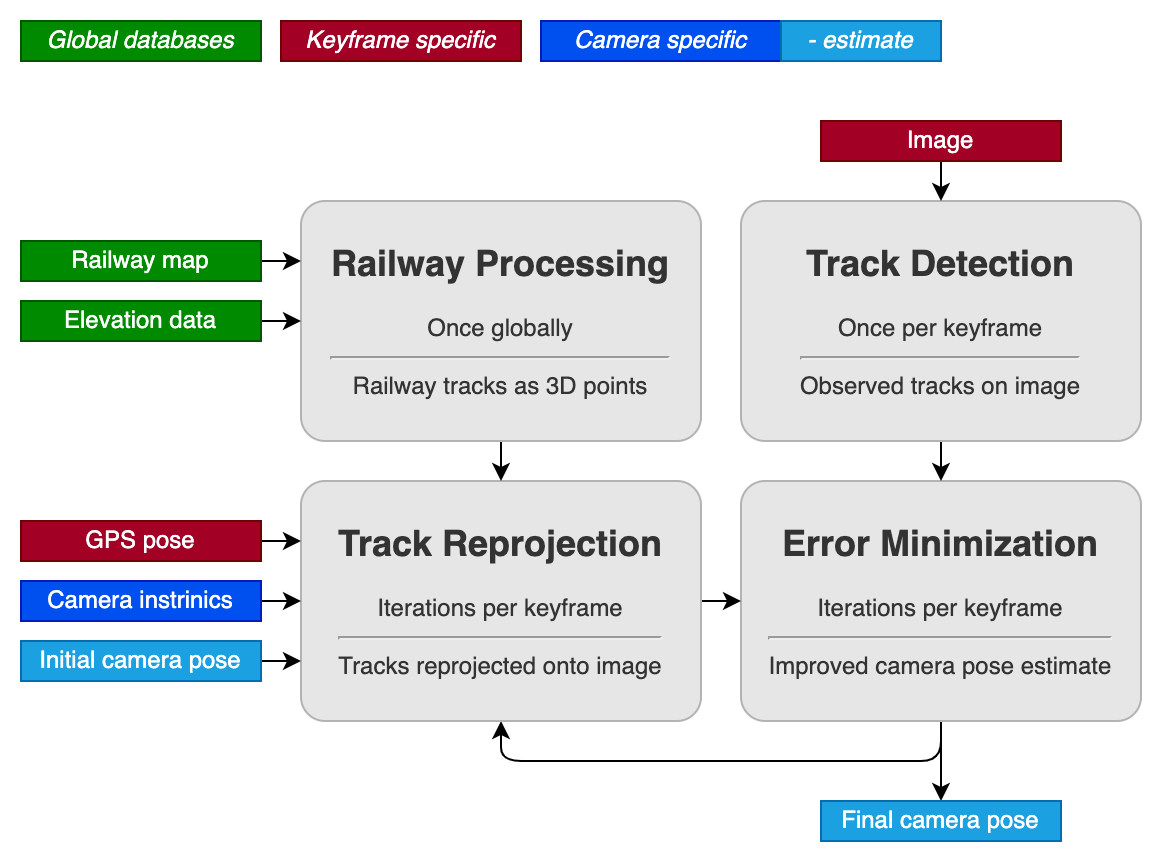
\includegraphics[width=\textwidth]{images/overview}
    \caption{Overview of main components, their interactions, and inputs/outputs.}
\end{center}
\end{figure}


\section{Railway Processing}
\label{sec:railway_processing}

At first, the nodes and tracks from the OSM file are converted into the data that is actually needed: 3D points of the railway tracks that are regularly spaced, a property that the OSM file does not fulfil.

Process list / pseudo-code / diagram

\begin{enumerate}
    \item Read OSM file
    \item Extract nodes and tracks
    \item Interpolate density of nodes
    \item ...
    \item Add elevation data to get 3D points
\end{enumerate}

\section{Track Reprojection}
\label{sec:track_reprojection}



\section{Track Detection}
\label{sec:track_detection}


\subsection{Railway Tracks}


\subsection{Poles}



\section{Error Minimization}
\label{sec:error_minimization}

